
\section{Convertidor reductor}
    \label{sec:buck_design}

    El sistema de carga multiquímica debe ser capaz de  proporcionar una 
    corriente constante para la carga de ambos tipos de baterías. Para ello
    se decidió emplear un convertidor reductor, el cual tiene por componente principal
    el circuito integrado LM2596. Para poder realizar un control del voltaje de salida ( y de
    forma indirecta la corriente del mismo)
    de forma electrónica, es decir aplicando un voltaje, se realizó una modificación al circuito
    de realimentación del circuito como es mostrado en la figura \ref{fig:buck_modificado}.

    \begin{figure}[H]
        \centering
        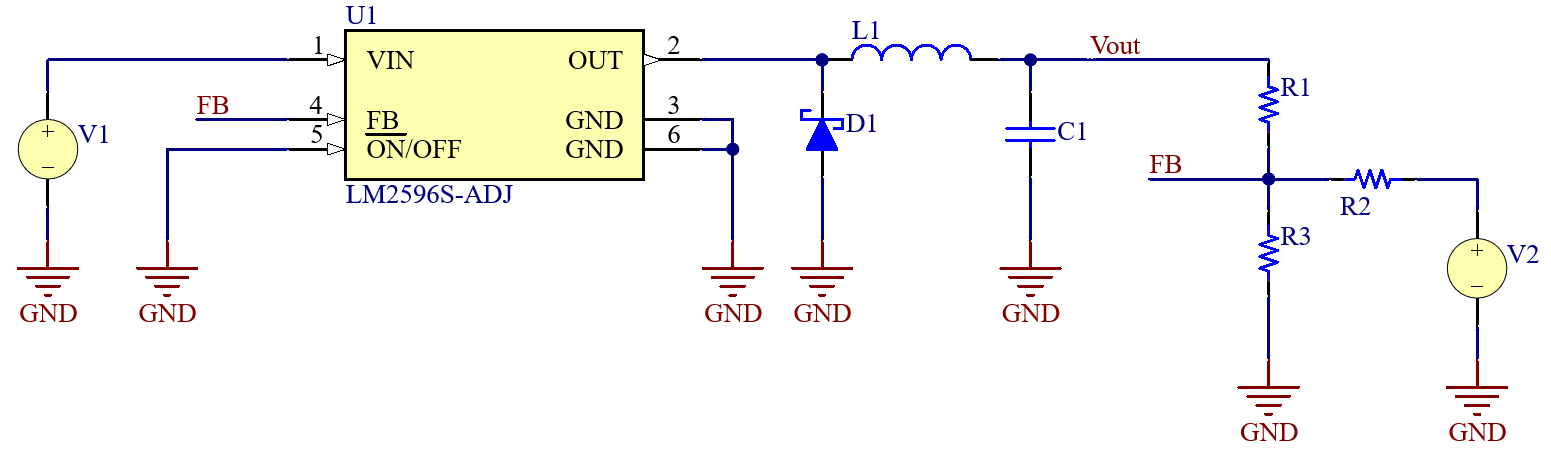
\includegraphics[scale=0.35]{imagenes/buck_control_simplificado.png}
        \caption{Convertidor reductor con realimentación modificación (versión simplificada) }
        \label{fig:buck_modificado}
    \end{figure}

    Para este convertidor se definieron los siguientes parámetros de rendimiento:

    $$ \Delta I = 150 \text{mA} $$
    $$ \Delta V = 1 \text{mV}$$

    Otros parámetros útiles para el diseño de este convertidor serán el voltaje
    de alimentación ($V_g$), así como la frecuencia de conmutación, $f_s$ (dada por la hoja 
    de datos del fabricante), los valores son:

    $$V_g = 12\text{V}$$
    $$ f_s = \frac{1}{T_s} = 150 \text{KHz}$$



    \subsection{Cálculo de resistencias para el circuito de retroalimentación}

    \label{sec:res_ret}

    Para poder determinar en que forma va a variar el voltaje en el nodo $V_{out}$ se realizó un 
    análisis de nodos en el nodo FB correspondiente a la figura \ref*{fig:buck_modificado}, 
    obteniendo la ecuación \ref*{eq:buck_control}.

    \begin{equation}
        V_{FB} = \frac{R_1R_2}{R_1R_2+R_3(R_1+R_2)} V_{out} + \frac{R_1R_3}{R_1R_3+R_2(R_1+R_3)} V_2
        \label{eq:buck_control}
    \end{equation}

    Donde $V_2$ el voltaje aplicado de forma externa para modificar el valor
    de voltaje a la salida. De la ecuación \ref*{eq:buck_control} se puede 
    observar que el valor de $V_{FB}$ es dependiente tanto de $V_2$ como de
    $V_{out}$. 

    Para determinar los valores de las resistencias se armó un sistema de dos ecuaciones,
    fijando los valores de $V_{FB}$,$V_{out}$,$V_2$, y $R_1$. Los dos valores necesarios
    de $V{out}$ se obtuvieron fijando el valor mínimo y máximo que podría tener a la salida
    el convertidor, los cuales fueron de $2.8\text{V}$ y $6.4\text{V}$ de forma que pueda usarse tanto para 
    cargar la celda de batería Li-ion, así como las 4 celdas NiMH. El valor de $V_{FB}$ 
    es el voltaje de referencia del IC LM2596. Los valores del voltaje de control se
    establecieron de forma que, cuando $V_2 = 5\text{V}$ el voltaje a la salida sea de 
    $2.8\text{V}$ mientras que cuando  $V_2 = 0\text{V}$ el voltaje sea de $6.4\text{V}$.
    Por último, se escogió un valor de $750\Omega$ para $R_1$ de forma arbitraria, siguiendo
    la recomendación de la hoja de datos del LM2596.

    Con lo explicado anteriormente, el sistema de ecuaciones a resolver es el siguiente:
    \begin{eqnarray}
        \frac{750R_3}{ 750R_3 + R_2(750 + R_3)} 6.4\text{V} = 1.23\text{V} \\
        \frac{750R_3}{ 750R_3 + R_2(750 + R_3)} 2.8\text{V} + \frac{750R_2}{750R_2+R_3(750+R_2)} 5\text{V} = 1.23\text{V}   
    \end{eqnarray}
    dando como resultado los siguientes valores para $R_2$ y $R_3$:

    $$R_2 = 2596.64\Omega$$ 
    $$R_3 = 3606.44\Omega$$

    Puesto que estos valores no son comerciales, se emplearon valores de resistencias en 
    paralelo, de forma que sea posible aproximar estos valores. Para el valor de $R_2$ 
    se empleó una resistencia de $3\text{K}\Omega$ y $20\text{K}\Omega$ dando como 
    resistencia equivalente $2.608\text{K}\Omega$. De igual forma se utilizó una 
    resistencia de $4.7\text{K}\Omega$ en paralelo con una de $15\text{K}\Omega$ para aproximar
    el valor de $R_3$, dando una resistencia total de $3.578\text{K}\Omega$.

    Al reemplazar en la ecuación \ref{eq:buck_control} los valores para $R_2$ y $R_3$ utilizados, 
    y dando un valor a $V_2$ de $5\text{V}$ se obtiene que el valor de $V_{out}$ es de $2.786\text{V}$
    mientras que si se reemplaza con $V_2 = 0\text{V}$ se obtiene que el valor de $V_{out}$ es de
    $6.431\text{V}$, los cuales son valores aceptables para la carga de ambas baterías,
    de forma que la variación en las resistencias no afecta significativamente
    el rango de operación del convertidor.

    \subsection{Componentes externos del convertidor}

        Los componentes externos necesarios para que el convertidor esté completo, son el 
        diodo $D_1$, el inductor $L_1$, y el capacitor $C_1$ que se muestran en la figura
        \ref{fig:buck_modificado}.

        Para $D_1$ se escogió el diodo 1N5817, el cual es un diodo \textit{
        schotky}, la elección de este componente fue debido a su baja caída de voltaje
        ($0.45\text{V}$ al conducir $1\text{A}$) lo cual minimiza las pérdidas por 
        conducción del mismo, mejorando la eficiencia del convertidor.

        Ya que el valor del inductor es dependiente
        del valor del voltaje a la salida del convertidor es necesario determinar cuál
        sería el valor óptimo. Para ello se definió la función $L(V)$ a partir de las 
        ecuaciones \ref{eq:ripple_L} y \ref{eq:salida_buck}. La función es la siguiente: 

        \begin{equation}
            L(V) = \frac{V_g - V}{2\Delta I}\frac{V}{V_g} T_s
            \label{eq:L_function}
        \end{equation}

        Posteriormente se obtuvo que el valor en
        donde la de derivada de $L(V)$ tiene un valor de cero es en $V = \frac{V_g}{2}$,
        por lo tanto, el valor máximo que tomará $L(V)$ será de 

        $$ L =  \frac{T_sV_g}{8\Delta I}$$
        
        Reemplazando los valores en la ecuación anterior se obtiene que el valor de 
        $L_1$ para el cual se asegura como máximo un rizado de $150 \text{mA}$ en 
        todo el rango de operación, es de $66.6 \mu \text{H}$, por lo que se usó un
        inductor de $68 \mu \text{H}$. Este aumento en el valor del inductor no afecta
        de manera negativa el funcionamiento del convertidor, ya que el valor calculado
        anteriormente unicamente es un límite inferior para el valor del inductor, un 
        valor mas alto reducirá a un mas el rizado en la corriente de salida, lo que 
        mejora el funcionamiento del convertidor.

        Por último, se empleó la ecuación \ref{eq:ripple_C} para obtener el valor 
        de $C_1$, siendo este de $125 \mu\text{F}$, por lo que se utilizó un capacitor
        electrolítico de $220 \mu\text{F}$ debido a que es el siguiente valor comercial 
        más alto disponible. De igual forma que con el inductor, el
        aumento en el valor del capacitor no afecta de manera negativa el funcionamiento
        del convertidor, ya que el valor calculado anteriormente es un límite inferior
        para el valor del capacitor, un valor más alto reducirá a un más el rizado en
        el voltaje de salida.

    \subsection{Componentes adicionales}

        Para asegurar un funcionamiento óptimo en \cite{lm2596}, se aconseja incorporar
        un capacitor en paralelo con la resistencia $R_2$ mostrada en la figura
        \ref{fig:buck_modificado}. La elección del valor de este condensador se basó
        en las pautas proporcionadas en el cuadro \ref{tb:feedforward_cap}. 
        Dado que el voltaje de salida mínimo es de $2.8\text{V}$, se optó por utilizar
        un capacitor de $33\text{nF}$.

        \begin{table}[H]
            \centering
            \begin{tabular}{|c|c|}
                \hline
                Voltaje de salida (V) & Capacitor \\
                \hline
                2 & $33\text{nF}$ \\
                4 & $10\text{nF}$ \\
                6 & $3.3\text{nF}$ \\
                9 & $1.5\text{nF}$ \\
                12 & $1\text{nF}$ \\
                15 & $680\text{pF}$ \\
                24 & $220\text{pF}$ \\
                28 & $220\text{pF}$ \\
                \hline
            \end{tabular}
            \caption{Valores para capacitancia de retroalimentación según \cite{lm2596}
                con respecto al voltaje de salida.}
            \label{tb:feedforward_cap}
        \end{table}



        Otro componente adicional necesario es un capacitor de desacople a la entrada
        del LM2596 para mejorar la estabilidad del voltaje de alimentación. Para su
        selección se empleó como criterio el uso de la figura \ref{fig:rms_cap}. Según
        \cite{lm2596} es necesario asegurar que el capacitor de salida pueda tolerar
        una corriente RMS entre el $50\%$ y $75\%$ de la corriente de salida.
        Para dar un mayor margen, se decidió escoger un capacitor que soporte una corriente
        RMS igual a la corriente máxima esperada, por lo que se escogió un capacitor
        de $470\mu\text{F}$ a $25\text{V}$.

        \begin{figure}[H]
            \centering

            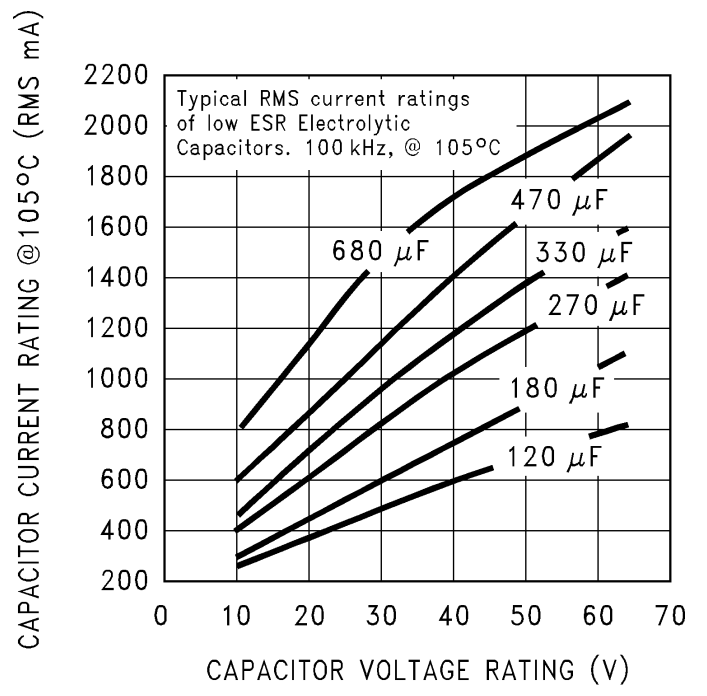
\includegraphics[scale=.4]{imagenes/rms_cap.png}
            \caption{capacidad de corriente RMS}
            \label{fig:rms_cap}

        \end{figure}

        Con todo lo discutido anteriormente, el diseño del convertidor reductor es mostrado
        en la figura \ref{fig:buck_finalizado}.

\begin{figure}[H]
    \centering

    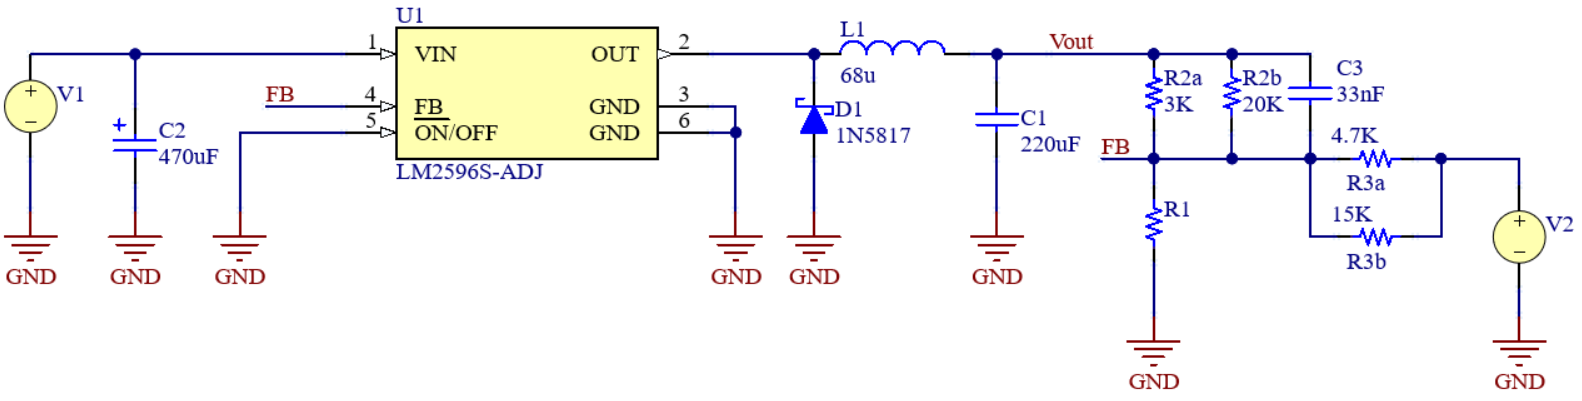
\includegraphics[scale=.45]{imagenes/buck_control_finalizado.png}
    \caption{Diseño del convertidor reductor finalizado}
    \label{fig:buck_finalizado}
\end{figure}

\subsection{Simulación del convertidor diseñado}

Para comprobar el correcto funcionamiento se realizó una simulación del 
convertidor diseñado. Para ello se empleó el simulador LTspice, junto con 
el modelo spice proporcionado por texas instruments para el circuito integrado
LM2596 (descarga disponible en \cite{noauthor_lm2596_nodate}). 

\begin{figure}[H]
    \centering
    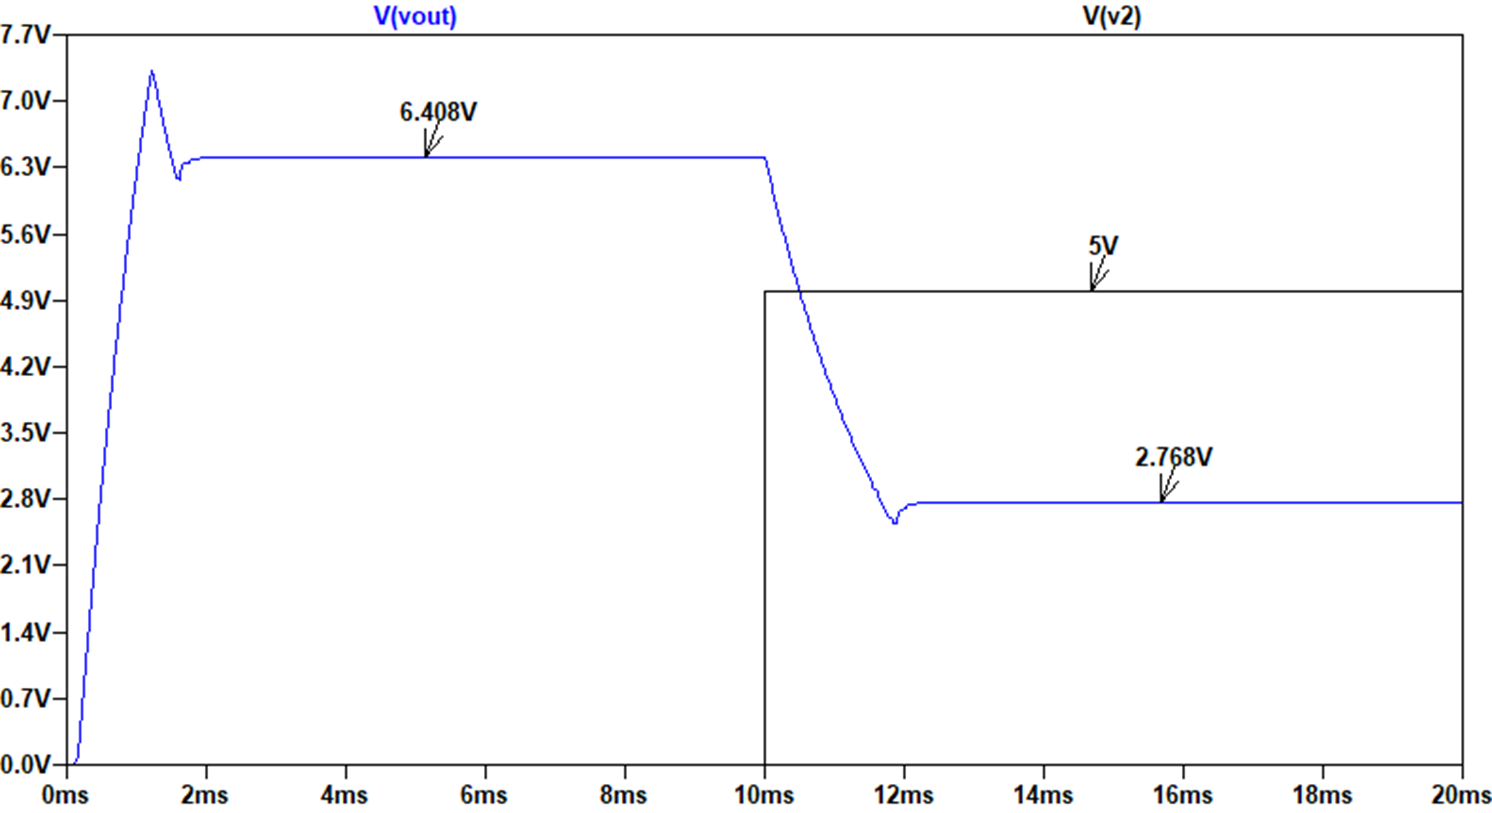
\includegraphics[scale=0.35]{imagenes/resultado_simulacion.png}
    \caption{Respuesta del convertidor (azul) contra el voltaje de control
            (negro).}
    \label{fig:sim_buck}
\end{figure}

En la figura \ref{fig:sim_buck} se muestra la respuesta del convertidor al
aplicar una señal escalón de $5\text{V}$ en la entrada de control. Se puede
observar que cuando el valor en el voltaje de control es de $0\text{V}$
la salida es de $6.408\text{V}$, además
cuando el valor del voltaje de control es de $5\text{V}$ el voltaje a la salida
del convertidor es de $2.768\text{V}$. Los cuales son valores cercanos a los esperados
al momento de realizar el diseño. 

Adicionalmente se puede observar que el rizado en el voltaje de salida del 
convertidor no es observable a la escala de voltaje en el que se está, esto debido
al uso de un valor más alto al calculado tanto para el inductor como para el 
capacitor del convertidor.

                                                                
\subsection{Prueba física del circuito}

Como último paso se realizó el diseño de un circuito impreso para probar el 
funcionamiento del circuito, en la figura \ref{fig:buck_pcb} se muestra la capa
superior e inferior del PCB.

\begin{figure}[H]
    \centering
    \begin{subfigure}{0.45\linewidth}
        \centering
        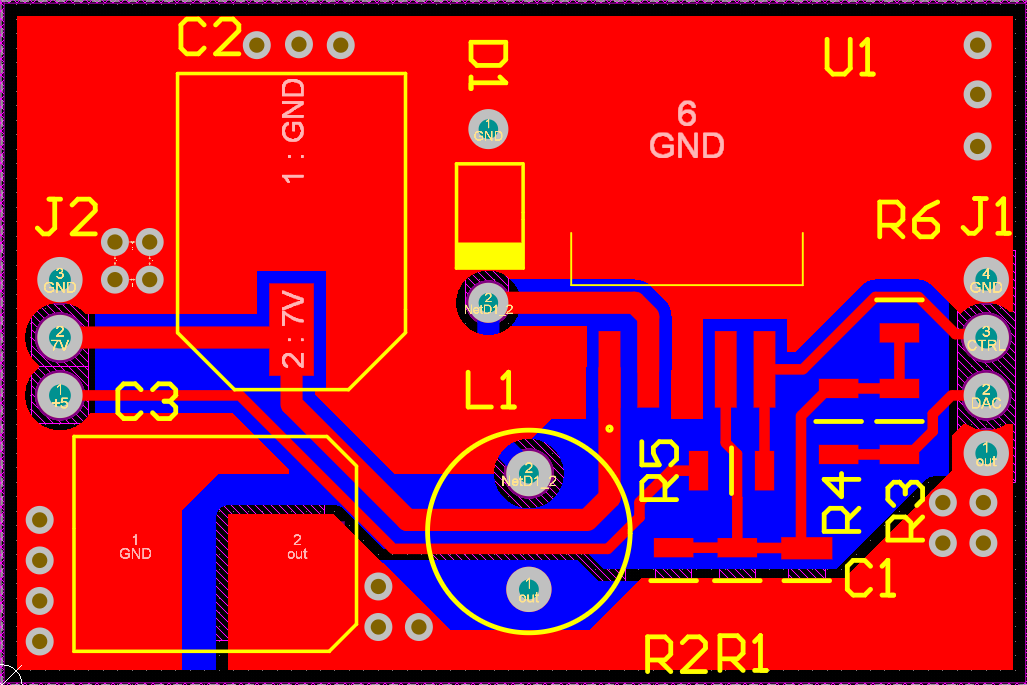
\includegraphics[scale=0.3]{imagenes/top_buck.png}
        \caption{Capa superior}
    \end{subfigure}
    \begin{subfigure}{0.45\linewidth}
        \centering
        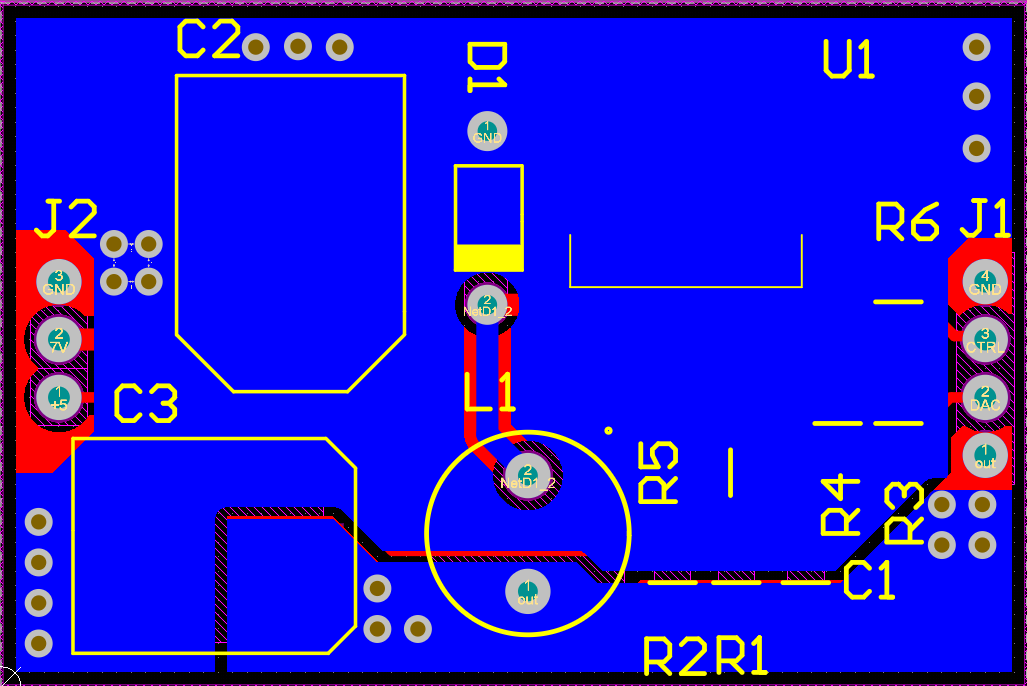
\includegraphics[scale=0.3]{imagenes/bottom_buck.png}
        \caption{Capa inferior}
    \end{subfigure}
    \vfill
    \begin{subfigure}{0.45\linewidth}
        \centering
        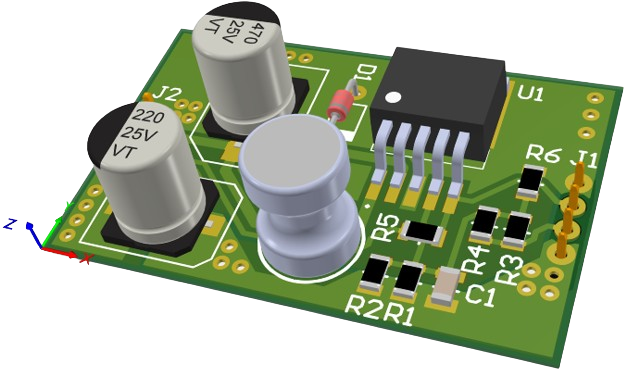
\includegraphics[scale=0.45]{imagenes/3d_buck.png}
        \caption{Vista 3D}
    \end{subfigure}
    \begin{subfigure}{0.45\linewidth}
        \centering
        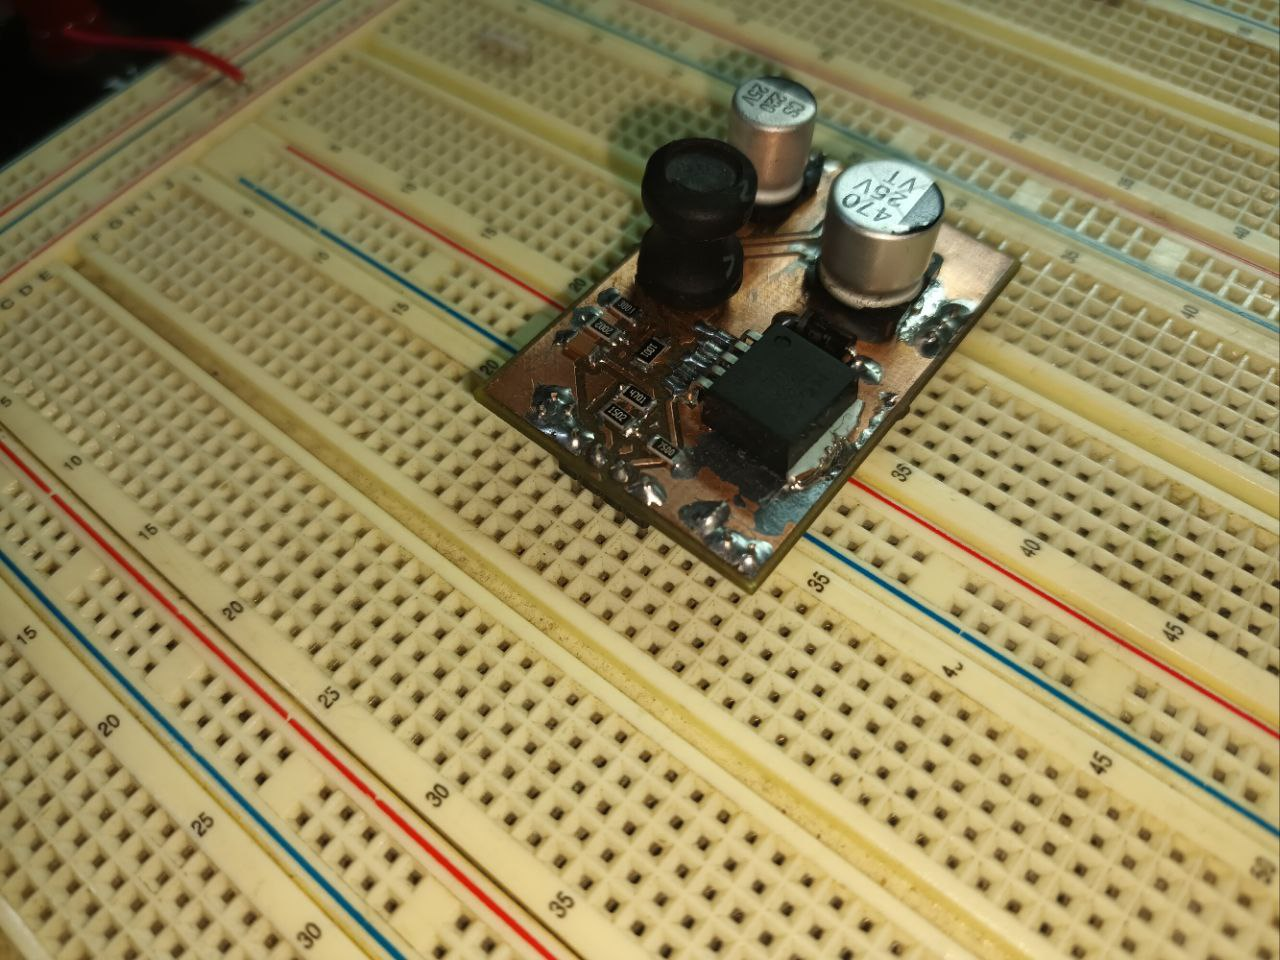
\includegraphics[scale=0.12]{imagenes/circuit_phis.jpg}
        \caption{PCB ensamblada}
    \end{subfigure}
    \caption{Diseño del PCB para el convertidor reductor}
    \label{fig:buck_pcb}
\end{figure}

Debido a que se manejan corrientes de hasta $1.5\text{A}$ es necesario que el
diseño del PCB sea capaz de manejar dicha corriente, para ello se empleó una 
calculadora de ancho de pistas \cite{noauthor_pcb_nodate}, con el cual se 
determinó que el ancho de las pistas debe ser de $0.53\text{mm}$ como mínimo,
esto tomando en cuenta que se estará usando un cobre con espesor de 1oz, y que
el maximo aumento de temperatura permitido es de 10\textordmasculine C. 

Se programó el microcontrolador ATmega328p para que genere una señal 
cuadrada de $5\text{V}$ con un periodo de 10 segundos en el pin PB1,
la cual se conectó a la entrada de control del convertidor. Al medir el voltaje
en la salida se obtuvo que el voltaje cuando se tienen $5\text{V}$ en la entrada
de control es de $2.76\text{V}$, mientras que cuando se tiene $0\text{V}$
en la entrada de control el voltaje a la salida es de $6.40\text{V}$, estos 
valores son cercanos a los esperados, por lo que el convertidor diseñado
funciona de forma correcta.

El circuito construido en protoboard para la prueba del convertidor se muestra
en la figura \ref{fig:prueba_buck}.

\begin{figure}[H]	
    \centering
    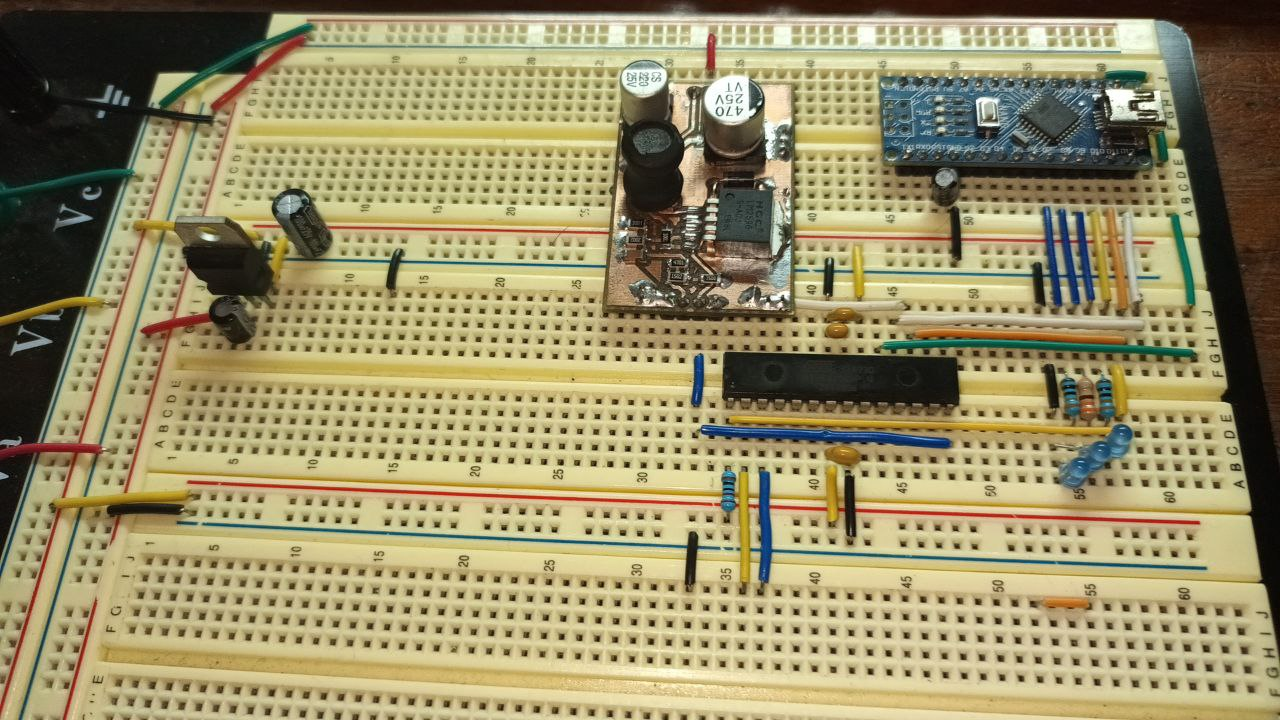
\includegraphics[scale=0.2]{imagenes/prueba_buck.jpg}
    \caption{Circuito para prueba del convertidor reductor (Arduino Nano únicamente
    es para programar el ATmega328p)} 
    \label{fig:prueba_buck}
\end{figure}

El código empleado en la prueba se muestra a continuación.

\begin{table}[H]
    \begin{lstlisting}
        #define F_CPU 8000000UL
        #include <avr/io.h>
        #include <util/delay.h>


        int main(void) {
                // ----     IO CONFIG  ---------
            DDRB = 0b00000011; // PB[7:2] input, PB1 out, PB0 out
            
            PORTB = 0b0000000; //activar PB0
            while (1) {
                PORTB |= 1<<1; //PB1 en 1
                _delay_ms(10000);
                PORTB &= ~(1<<1); //PB1 en 0
                _delay_ms(10000);
            }
        }

    \end{lstlisting}
    \caption{Código para prueba del convertidor reductor}
\end{table}
